\chapter{Implementación y análisis de algoritmos}

En este apartado se realizará un análisis detallado sobre cómo funciona cada uno de los algoritmos seleccionados para el estudio desde un punto de vista teórico. Se explicarán las técnicas que utiliza cada uno para llegar a la solución óptima y cómo se asemejan dichas técnicas al comportamiento humano, para de ese modo poder considerarse un algoritmo socioinspirado. Además, se arrojarán detalles destacados de la implementación de cada uno en particular, si dicha implementación así lo requiriese.

Los algoritmos se analizarán en orden cronológico, siendo el más antiguo de todos Imperialist Competitive Algorithm (2007) \cite{ica-conference} y el más reciente Ideology Algorithm (2016) \cite{ia-article}.

\section{Detalles generales sobre la implementación}

En primer lugar, antes de comenzar con la explicación de los algoritmos, conviene dar una visión general acerca de la implementación en este estudio, cómo se ha llevado a cabo y con qué herramientas.

Los algoritmos se han implementado utilizando el lenguaje de programación \textbf{Python} en su versión 3.6 \cite{python-3.6-doc}, elección personal del alumno, dada su facilidad para trabajar con vectores y matrices utilizando librerías como \textbf{Numpy} \cite{numpy-doc}, además de otras de representación gráfica como \textbf{Matplotlib} \cite{matplotlib-doc}. Poder operar de forma sencilla con múltiples matrices que habitualmente constituirán la población de soluciones de cada problema resultó un detalle determinante para tomar la decisión.

Encontrar el código fuente de los algoritmos mencionados resulta una ardua tarea, ya que la mayoría de los autores no liberan su código en ninguna plataforma. En algunas ocasiones es posible encontrar versiones en el lenguaje de programación \textbf{MATLAB}, uno de los lenguajes más utilizados en el ámbito científico y de investigación por su capacidad de cómputo y de operar con fórmulas matemáticas de gran dimensión. Sin embargo, MATLAB es un software privativo y de pago, y el alumno ha querido liberar su proyecto desde el primer momento, por lo que se rechazó la idea de implementarlos en este lenguaje. Sin embargo, sí que se ha utilizado como referencia para algún algoritmo una versión de MATLAB sobre la que basar la implementación en Python.

En relación a lo comentado en el párrafo anterior, el proyecto ha estado libre y alojado en la plataforma \textbf{GitHub} \cite{repositorio-tfg} desde que se comenzó la implementación, para que cualquier usuario interesado pudiese no sólo acceder a él sino también comprobar cómo está hecho, y en un futuro incluso realizar los cambios pertinentes que considerase, cumpliendo así el paradigma del software libre.

\section{Imperialist Competitive Algorithm (ICA)}

El primer algoritmo a analizar, \textbf{Imperialist Competitive Algorithm} o, según sus siglas, \textbf{ICA}, fue presentado por primera vez en 2007 por Atashpaz-Gargari y Lucas \cite{ica-conference}. Se trata de un algoritmo que podría ser agrupado en la subcategoría de socioinspirados basados en conquistas y colonialismo, como se procede a explicar.

La implementación del ICA en Python no pudo ser encontrada en internet, sin embargo sí que se encontró el código fuente en MATLAB, subido por el propio autor del \textit{paper} \cite{ica-matlab}. Este código se ha usado como referencia para implementarlo de forma similar en Python, ya que algunos detalles varían con respecto a la literatura.

Este algoritmo parte de la idea de un mundo completamente colonialista, plagado de países que luchan por alzarse vencedores y conquistadores. En esta guerra constante, los países con más poder se volverían los líderes, y podrían contar con numerosas colonias a su servicio. Por otra parte, aquellos países que no pueden vencer a los demás se verían relegados a ocupar un puesto de colonia para siempre.

Durante la guerra también se puede producir una revolución o alzamiento de una de las colonias contra su propio imperio. Si esta colonia resulta ser más poderosa que el actual líder, dicha posición pasa a ser suya. También puede darse el caso totalmente opuesto; si una colonia resulta realmente débil, un imperio colindante puede absorberla y hacerse más fuerte gracias a ella. Y por supuesto, un imperio puede ser colonizado al completo por otro, haciéndose así cargo de sus colonias restantes y del propio país imperial.

En palabras de los propios autores del algoritmo, <<la competición imperialista con suerte convergerá a un estado en el que sólo haya un imperio y todas sus colonias se hallen en la misma posición y tengan el mismo coste que el país imperialista>>.

Como se puede observar de esta hoja de ruta del algoritmo, la relación con la sociedad es evidente, aunque recuerde más a épocas pasadas que a la actualidad. Este es el funcionamiento del algoritmo a grandes rasgos, pero a continuación se detallarán las características más llamativas del mismo. Previamente se muestra un pseudocódigo del algoritmo, para ayudar a comprender cada paso del mismo antes de la explicación detallada.

\begin{algorithm}
	\caption{Imperialist Competitive Algorithm}
	\begin{algorithmic}[1]
		\State $imperios \gets \textit{inicializarImperios()}$
		\While{\textbf{not} \textit{criterioParada}}
		\For{\textbf{each} \textit{colonia}}
		\State $colonia \gets colonia + (imperialista - colonia + rand())$
		\If{$peso(colonia) < peso(imperialista)$}
		\State $imperialista \gets colonia$
		\EndIf
		\EndFor
		\State $imperios \gets competicionImperial()$
		\If{\textbf{any} \textit{imperio} \textbf{is empty}}
		\State $imperios \gets eliminarImperio(imperio)$
		\EndIf
		\EndWhile
		\State{\textbf{return} \textit{min(peso(imperialistas))}}
	\end{algorithmic}
\end{algorithm}

Se puede comenzar este análisis en base a los distintos componentes del algoritmo, relacionándolos con la descripción anterior y comprobando por qué se trata de técnicas socioinspiradas.

En primer lugar conviene hablar acerca de la población. Si bien habitualmente en estos algoritmos socioinspirados la población suele estar constituida de individuos, siendo esta una agrupación de los mismos, en el caso del algoritmo ICA no es así. En este algoritmo se realiza un símil con una sociedad global donde cada una de las soluciones que compone la población es como un país, o en este caso como una colonia. Por tanto, la figura del ser humano como persona individual no aparece en esta propuesta.

Una vez que se han instanciado las primeras soluciones o colonias que ocuparán la población inicial, hay que seleccionar aquellas que sean más poderosas para considerarlas <<imperialistas>>, es decir, serán los líderes de cada uno de los imperios en los que se divida el problema. Por supuesto, tanto el número de colonias como el número de imperios iniciales son definidos en los parámetros del algoritmo y pueden variar si así se desea.

A lo largo de todo este algoritmo se entenderá que un país es más poderoso que otro si \textbf{su evaluación para la función objetivo es menor}, dado que se trata de problemas de optimización buscando el menor valor posible. La asignación de los imperios se hace con respecto a las colonias iniciales con un menor valor para dicha función.

Con los imperios constituidos y las colonias distribuidas se comienza a desarrollar el bucle principal del algoritmo, que finalizará cuando se cumpla el criterio de parada. La implementación de este algoritmo originalmente paraba tras un número de <<décadas>> (iteraciones del bucle principal), pero a fin de integrarlo con el resto de algoritmos del estudio se añadió la posibilidad de definir un criterio de parada por número de evaluaciones de la función objetivo.

En cada iteración de dicho bucle cada colonia realiza un desplazamiento hacia su imperialista. El desplazamiento tiene un componente de aleatoriedad que permite que no converjan todas las soluciones en el primer imperialista nada más comenzar las iteraciones. A continuación se puede observar una representación gráfica de dicho movimiento.

\begin{figure}[h]
	\centering
	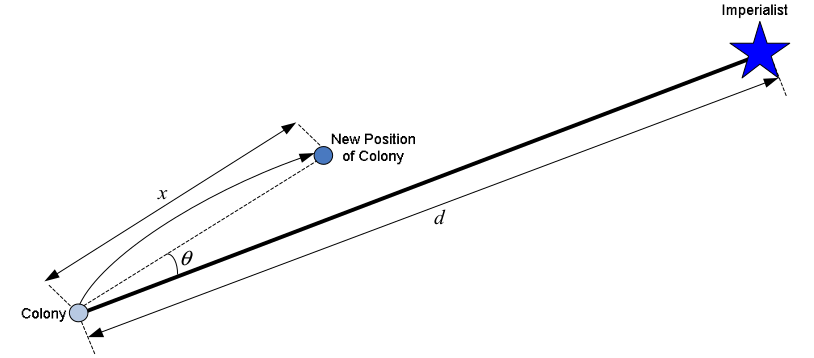
\includegraphics[scale=0.4]{imagenes/ica-desplazamiento.png}
	\caption{Desplazamiento de una colonia hacia su imperialista, con un componente de aleatoriedad \cite{ica-conference}.}
	\label{ica-desplazamiento}
\end{figure}

El movimiento producido $x$ queda definido por la siguiente fórmula

\begin{equation}\label{ica-eq-desplazamiento1}
x \sim U(0, \beta \times d)
\end{equation}

en la cual $d$ es la distancia entre la colonia y el imperialista y $\beta$ representa el llamado <<coeficiente de asimilación>>. Es decir, se trata de un desplazamiento hacia el imperialista donde la distancia recorrida está definida por un valor uniforme aleatorio entre 0 y la máxima distancia.

Además, el ángulo $\theta$ que aparece en la figura, que desvía a la colonia de su dirección, viene calculado de la siguiente forma

\begin{equation}\label{ica-eq-desplazamiento2}
	\theta \sim U(-\gamma, \gamma)
\end{equation}

donde $\gamma$ es el parámetro que ajusta la desviación de la dirección, y que es llamado por los autores <<coeficiente del ángulo de asimilación>>.

Los cambios producidos mediante estos operadores mencionados ayudan a diversificar las posiciones de las colonias y a que no se agrupen automáticamente en torno a la mejor solución del imperio. Esto permite al algoritmo explorar el espacio de búsqueda adecuadamente y no caer en posibles óptimos locales con facilidad en las primeras iteraciones, lo que limitaría mucho el proceso evolutivo. Si la nueva posición hacia la que se mueve una colonia resulta ser mejor que la del actual imperialista de dicho imperio, se intercambian los puestos y el resto de colonias intentará moverse hacia la nueva mejor solución.

La competición imperialista que tiene lugar en cada iteración del bucle principal aporta aún más variedad al proceso, llevando a la peor de las colonias del peor imperio hasta el imperio que más probabilidad tiene de adquirirla, que suele ser el más poderoso. Este poder de los imperios se calcula en función del peso del imperialista y del peso medio de sus colonias. Esta decisión también aporta más variedad a la par que realismo en el proceso imperialista, ya que si un el país líder del imperio es muy poderoso pero tiene muchas colonias débiles, generalmente dicho imperio será menos potente que uno que tenga un imperialista algo peor y menos colonias aunque más fuertes.

Una vez que un imperio se quede sin colonias, este pasa a ser absorbido por el imperio más fuerte, y la cantidad de imperialistas se reduce. El proceso se repite en cada iteración del bucle hasta que quede solamente un imperio que contenga todas las colonias; en tal caso, a partir de esa iteración en el bucle principal solamente se moverán las colonias hacia nuevas posiciones, tratando de explorar las cercanías del país imperialista.

Como se ha mencionado antes, en el código fuente que el autor subió a la página \textbf{MathWorks} \cite{ica-matlab} hay algunos detalles que cambian con respecto al paper, y que se han añadido en la implementación en Python. En este caso se trata de un componente de revolución que puede afectar a algunas colonias en cada iteración, y que permite que cambien radicalmente de posición. Gracias a este componente aleatorio se podría llegar a explorar una zona del espacio de búsqueda a la que no se haya llegado anteriormente y que aporte una mejor solución.

Para concluir el análisis del ICA, se puede afirmar con certeza que basa muchísimo su comportamiento en los algoritmos de \textbf{Particle Swarm Optimization (PSO)}. En este caso, cada imperio funcionaría como un algoritmo PSO en sí, siendo las partículas las colonias y la mejor posición la del país imperialista. La principal variación consiste en que el algoritmo simula varios PSO compitiendo entre sí, aunque mezclando sus partículas mediante revoluciones o intercambiándolas en el proceso. La propuesta es interesante y una de las primeras en aportar un enfoque colonialista al planteamiento del algoritmo, por lo que resultó especialmente interesante para el estudio.

El punto crítico al algoritmo viene en torno a la exploración del espacio de búsqueda. Para ello es necesario distinguir bien en este caso cuál es la fase de exploración y cuál la de explotación. En este algoritmo se produce una exploración del espacio de búsqueda cuando hay varios imperios, y además las colonias del imperio se encuentran suficientemente separadas del imperialista como para que su avance hacia él permita valorar un considerable número de posiciones en los alrededores, pero no en las inmediaciones. Esta búsqueda en las posiciones más cercanas a la mejor solución es la que se considera la explotación, cuyo principal objetivo es comprobar si en las cercanías hay alguna posibilidad de mejora para apuntillar la solución. Esta fase suele darse en las iteraciones más avanzadas del algoritmo, cuando ya se tiene más o menos claro dónde puede estar el óptimo.

Si bien se ha comentado lo interesante de la propuesta para que no se caiga de inmediato en óptimos locales y la ventaja que aporta que cada colonia tenga posibilidad de revolucionarse y dar lugar a una nueva exploración, el problema es que una o dos colonias colocadas de forma aleatoria no suponen una exploración decente. Tener pronto todas las colonias agrupadas en un mismo imperio supone contar con una fase de exploración corta, lo que hace bastante factible la posibilidad de que el algoritmo se quede en un óptimo local y no vuelva a moverse de ahí ya que el resto de las iteraciones implican casi esencialmente una fase de explotación.